\documentclass[12pt, a4paper]{article}

\usepackage[T1]{fontenc}
\usepackage[utf8]{inputenc}
\usepackage[charter, cal=cmcal]{mathdesign}
\usepackage[scaled=0.92]{helvet}
\usepackage{geometry}
\geometry{a4paper, top=30mm, bottom=30mm, inner=30mm, outer=30mm}

\usepackage{amsmath, amsthm}
\usepackage{amssymb}
\usepackage{xcolor}
\usepackage{tikz}
\usetikzlibrary{arrows.meta, calc, shapes.geometric}
\usepackage{fancyhdr}
\usepackage{titlesec}
\usepackage{enumitem}
\usepackage{booktabs}
\usepackage{array}
\usepackage{parskip}
\usepackage[colorlinks=true, linkcolor=NavyBlue, urlcolor=NavyBlue, citecolor=NavyBlue]{hyperref}

% ── Colours (Journey 6 — navy blue / gold) ────────────────────────────────────
\definecolor{NavyBlue}{HTML}{1E3A8A}
\definecolor{ModuleColor}{HTML}{2563EB}
\definecolor{PuzzleColor}{HTML}{D97706}
\definecolor{DiscoveryColor}{HTML}{B45309}
\definecolor{ProblemColor}{HTML}{6B21A8}
\definecolor{ReflectColor}{HTML}{0D9488}
\definecolor{LightBlue}{HTML}{EFF6FF}
\definecolor{LightGold}{HTML}{FEF3C7}
\definecolor{LightGreen}{HTML}{ECFDF5}

% ── Custom Environments (No TColorBox for Math style) ─────────────────────────
\newenvironment{puzzlebox}
  {\par\medskip\fillcolorbox{LightGold}{PuzzleColor}{The Puzzle}}
  {\par\medskip}

\newenvironment{discoverybox}
  {\par\medskip\fillcolorbox{LightGreen}{DiscoveryColor}{Discovery}}
  {\par\medskip}

\newenvironment{namedconcept}[1]
  {\par\medskip\fillcolorbox{LightBlue}{NavyBlue}{#1}}
  {\par\medskip}

\newenvironment{reflectionbox}
  {\par\medskip\fillcolorbox{LightBlue}{ReflectColor}{Reflection}}
  {\par\medskip}

\newcommand{\fillcolorbox}[3]{%
  \noindent
  \filldrawbox{#1}{#2}{\textbf{\sffamily\color{white}#3}}\par\nobreak\vspace{4pt}
}

\newcommand{\filldrawbox}[3]{%
  \colorbox{#1}{\parbox{\dimexpr\linewidth-2\fboxsep\relax}{%
    \vspace{4pt}\noindent\hspace{4pt}#3\vspace{4pt}%
  }}%
}

% ── Section formatting ────────────────────────────────────────────────────────
\titleformat{\section}
  {\normalfont\sffamily\Large\bfseries\color{NavyBlue}}
  {\thesection}{1em}{}[\color{NavyBlue!40}{\titlerule[1.5pt]}]
\titleformat{\subsection}
  {\normalfont\sffamily\large\bfseries\color{ModuleColor}}{\thesubsection}{1em}{}

\pagestyle{fancy}
\fancyhf{}
\fancyhead[L]{\small\sffamily\color{NavyBlue}\textit{Discovery Curriculum}}
\fancyhead[R]{\small\sffamily\color{ModuleColor}\textit{Journey 6 $\cdot$ Module 1}}
\fancyfoot[C]{\small\color{NavyBlue}\thepage}
\renewcommand{\headrulewidth}{0.4pt}

\newcommand{\newterm}[1]{\textit{\textcolor{DiscoveryColor}{#1}}}

\begin{document}

\thispagestyle{empty}
\begin{center}
{\small\color{ModuleColor}\textbf{DISCOVERY CURRICULUM}\quad$\cdot$\quad\textbf{JOURNEY 6: ABSTRACTION}}
\vspace{0.6cm}

{\color{NavyBlue}\rule{\linewidth}{2.5pt}}\vspace{0.5cm}

{\Huge\bfseries\color{NavyBlue}Module 1}\\[0.3cm]
{\LARGE\bfseries\color{ModuleColor}Group Theory and Symmetry}\\[0.4cm]
{\color{PuzzleColor}\rule{0.4\linewidth}{1.5pt}}\\[0.4cm]
{\large\itshape\color{NavyBlue!80}
A geometric object remains invariant under transformations.\\[0.15cm]
The set of these transformations forms a closed structure.\\[0.15cm]
This structure is the algebraic definition of symmetry.}

\vspace{1cm}
\begin{tabular}{rl}
\textbf{Journey}         & Journey 6 --- Abstraction \\[4pt]
\textbf{Module}          & 1 of 4 \\[4pt]
\textbf{Prerequisites}   & Journey 1 (relations), Journey 3 (linear transformations) \\[4pt]
\textbf{You will discover} & Groups, subgroups, Cayley tables, Lagrange's Theorem, homomorphisms \\[4pt]
\textbf{Format}          & 8 problems $+$ 2 deep problems $\approx$ 12 pages \\
\end{tabular}
\vspace{1cm}

{\color{NavyBlue}\rule{\linewidth}{2.5pt}}
\end{center}

\newpage

\section{Module 6.1 --- Group Theory and Symmetry}
\label{sec:mod6.1}

\subsection*{Motivation}

In our study of mathematics so far, we have focused on concrete structures: numbers (Journey 1), limits and rates (Journey 2), vectors and matrices (Journey 3), and fields and coordinate spaces (Journey 4).
Now, we step back to examine structure in its purest, most abstract form.

We begin with the concept of **symmetry**.
Symmetry is not merely a visual aesthetic. It is a mathematical property: invariance under a set of transformations.
Whether we are rotating a triangle in a plane, permuting the roots of a polynomial, or changing the reference frame of a quantum mechanical observer, we are performing operations that leave some property invariant.
The algebra that governs these operations is **Group Theory**.
This module formalizes this algebra, proving fundamental theorems that restrict the possible structures of symmetry.

\subsection{The Symmetries of the Triangle}

We investigate the geometric operations that leave a regular polygon invariant.

\begin{puzzlebox}
Consider an equilateral triangle with vertices labeled 1, 2, and 3.
We define a **symmetry operation** as any rigid motion of the plane that maps the triangle back onto itself.
* Let $r$ be a counterclockwise rotation of $120^\circ$ about the center.
* Let $s$ be a reflection across the vertical axis passing through vertex 1 and the midpoint of the opposite side.

\begin{center}
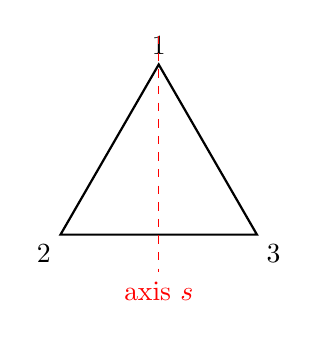
\begin{tikzpicture}[scale=1.2]
  \coordinate (A) at (90:1.2);
  \coordinate (B) at (210:1.2);
  \coordinate (C) at (330:1.2);
  \draw[thick] (A) -- (B) -- (C) -- cycle;
  \node[above] at (A) {1};
  \node[below left] at (B) {2};
  \node[below right] at (C) {3};
  \draw[dashed, red] (90:1.5) -- (270:1.0) node[below] {axis $s$};
\end{tikzpicture}
\end{center}

\begin{enumerate}[label=(\alph*), leftmargin=*]
  \item Show that there are exactly 6 symmetry operations for the equilateral triangle: three rotations (including the $0^\circ$ rotation) and three reflections.
  \item If we perform rotation $r$ and then reflection $s$, we denote the composition as $s \circ r$ (or simply $sr$).
        Show that the composition of any two operations in our set is equivalent to a single operation in the same set.
  \item Verify that composition is not commutative: $sr \neq rs$. Explain this geometrically.
\end{enumerate}
\end{puzzlebox}

\subsection{The Axioms of a Group}

We abstract the properties of symmetry compositions into a formal algebraic structure.

\begin{namedconcept}{The Group Axioms}
A \newterm{group} is a set $G$ together with a binary operation $*$ (which maps any pair $a, b \in G$ to an element $a * b \in G$) that satisfies the following four axioms:
1. **Closure:** For all $a, b \in G$, $a * b \in G$.
2. **Associativity:** For all $a, b, c \in G$, $(a * b) * c = a * (b * c)$.
3. **Identity:** There exists an element $e \in G$ such that $e * a = a * e = a$ for all $a \in G$.
4. **Inverse:** For each $a \in G$, there exists an element $a^{-1} \in G$ such that $a * a^{-1} = a^{-1} * a = e$.

If $a * b = b * a$ for all $a, b \in G$, the group is called \newterm{abelian} (or commutative).
\end{namedconcept}

\begin{enumerate}[label=(\alph*), leftmargin=*]
  \item Show that the set of integers $\mathbb{Z}$ under addition forms an abelian group. What is the identity element? What is the inverse of $x$?
  \item Show that the set of non-zero real numbers $\mathbb{R} \setminus \{0\}$ under multiplication forms an abelian group.
  \item Explain why the set of $n \times n$ invertible matrices under matrix multiplication forms a non-abelian group. (This is the **General Linear Group**, $GL_n(\mathbb{R})$).
\end{enumerate}

\subsection{Subgroups and Lagrange's Theorem}

We study structures within groups and the mathematical constraints on their sizes.

\begin{namedconcept}{Subgroups and Cosets}
Let $G$ be a group under $*$. A subset $H \subseteq G$ is a \newterm{subgroup} (denoted $H \le G$) if $H$ is itself a group under $*$.
* **The Subgroup Criterion:** A non-empty subset $H \subseteq G$ is a subgroup if and only if for all $a, b \in H$, $a * b^{-1} \in H$.
* **Cosets:** If $H \le G$, the **left coset** of $H$ associated with an element $g \in G$ is the set:
  \[
    gH \;=\; \{g * h : h \in H\}.
  \]
\end{namedconcept}

The number of elements in a group $G$ is called its \newterm{order}, denoted $|G|$.
\begin{enumerate}[label=(\alph*), leftmargin=*]
  \item **Lagrange's Theorem:** If $G$ is a finite group and $H$ is a subgroup of $G$, then the order of $H$ must divide the order of $G$:
  \[
    |G| \;=\; [G:H] \cdot |H|,
  \]
  where $[G:H]$ is the number of distinct left cosets of $H$ in $G$ (the **index** of $H$).
  \item Let the group of symmetries of the triangle be $D_3$, with $|D_3| = 6$.
        According to Lagrange's theorem, what are the only possible orders of subgroups of $D_3$?
  \item Find a subgroup of $D_3$ of order 2, and another of order 3.
\end{enumerate}

\subsection{Homomorphisms and Isomorphisms}

We study the mappings that preserve algebraic structure, allowing us to identify when two seemingly different groups are structurally identical.

\begin{namedconcept}{Homomorphisms}
A mapping $\phi: G \to H$ between two groups $(G, *)$ and $(H, \cdot)$ is a \newterm{homomorphism} if it preserves the group operation:
\[
  \phi(a * b) \;=\; \phi(a) \cdot \phi(b) \qquad \text{for all } a, b \in G.
\]
If $\phi$ is also a bijection (one-to-one and onto), it is called an \newterm{isomorphism} (denoted $G \cong H$).
\end{namedconcept}

\begin{enumerate}[label=(\alph*), leftmargin=*]
  \item Prove that if $\phi: G \to H$ is a homomorphism, then $\phi(e_G) = e_H$, and $\phi(a^{-1}) = \phi(a)^{-1}$.
  \item Show that the exponential mapping $\phi(x) = e^x$ is an isomorphism from the group of real numbers under addition $(\mathbb{R}, +)$ to the group of positive real numbers under multiplication $(\mathbb{R}^+, \cdot)$.
  \item Why is this isomorphism the mathematical reason why slide rules can perform multiplication by adding distances?
\end{enumerate}

\newpage

\section{Part 3 --- Discovery}

\begin{discoverybox}
\textbf{What have we built?}

\textbf{First.} A group is an axiomatic algebraic structure (closure, associativity, identity, inverse) that formalizes the composition of transformations.

\textbf{Second.} The symmetries of regular polygons are governed by the Dihedral groups $D_n$, which are non-abelian for $n \ge 3$.

\textbf{Third.} Lagrange's Theorem restricts the possible size of subgroups, stating that the order of any subgroup $H$ must divide the order of the parent group $G$. This arises because the cosets of $H$ partition $G$ into equal-sized disjoint subsets.

\textbf{Fourth.} Homomorphisms are mappings that preserve the algebraic structure of groups. Isomorphisms show that two groups are structurally identical, regardless of their notation or elements.
\end{discoverybox}

\newpage

\section{Part 4 --- What This Is Called}

\begin{namedconcept}{Algebraic Group Parameters}
* **Abelian Group:** A group in which the operation is commutative ($a*b = b*a$).
* **Dihedral Group ($D_n$):** The group of symmetries of a regular $n$-sided polygon, of order $2n$.
* **Lagrange's Theorem:** The theorem stating that for any finite group $G$, the order of any subgroup $H$ divides the order of $G$.
* **Coset:** A set formed by multiplying every element of a subgroup by a fixed element of the parent group.
* **Isomorphism:** A bijective map between two groups that preserves the group operations, proving structural equivalence.
\end{namedconcept}

\newpage

\section{Part 5 --- Solved Exercises}

\begin{enumerate}[label=\textbf{E\arabic*.}]
  \item \textbf{Uniqueness of Identity and Inverse.}
  
        Prove that in any group $G$:
        (a) The identity element $e$ is unique.
        (b) For any $a \in G$, its inverse $a^{-1}$ is unique.
        
        \textbf{Solution:}
        (a) Suppose there are two identity elements $e$ and $e'$ in $G$.
        By the definition of an identity element, since $e'$ is an identity:
        \[
          e * e' \;=\; e.
        \]
        Similarly, since $e$ is an identity:
        \[
          e * e' \;=\; e'.
        \]
        Equating the two expressions for $e * e'$, we get:
        \[
          e \;=\; e'.
        \]
        Thus, the identity element is unique.
        
        (b) Suppose $a$ has two inverses, $b$ and $c$, in $G$.
        By the definition of an inverse:
        \[
          a * b \;= \; b * a \;=\; e, \qquad \text{and} \qquad a * c \;=\; c * a \;=\; e.
        \]
        Now, evaluate the composition $b * a * c$ using associativity:
        \[
          (b * a) * c \;=\; e * c \;=\; c.
        \]
        Alternatively:
        \[
          b * (a * c) \;=\; b * e \;=\; b.
        \]
        By associativity, $(b * a) * c = b * (a * c)$, which immediately yields:
        \[
          b \;=\; c.
        \]
        Thus, the inverse of any element $a$ is unique.
        
  \item \textbf{Abelian Property from Self-Inverse.}
  
        Prove that if every element $a$ in a group $G$ satisfies $a^2 = e$ (meaning $a = a^{-1}$), then $G$ must be abelian.
        
        \textbf{Solution:}
        Let $x$ and $y$ be any two elements in $G$.
        We wish to show that $x * y = y * x$.
        
        By the given hypothesis, every element in $G$ is its own inverse.
        Therefore, for $x$, $y$, and the composed element $x * y$:
        \[
          x^{-1} \;=\; x, \qquad y^{-1} \;=\; y, \qquad \text{and} \qquad (x * y)^{-1} \;=\; x * y.
        \]
        Now, we use the general property of group inverses for compositions:
        \[
          (x * y)^{-1} \;=\; y^{-1} * x^{-1}.
        \]
        Substitute the self-inverse properties into both sides of this relation:
        \[
          x * y \;=\; y * x.
        \]
        Since this holds for all $x, y \in G$, the group $G$ is abelian.
\end{enumerate}

\newpage

\section{Part 6 --- Problems}

\begin{enumerate}[label=\textbf{P\arabic*.}]
  \item \textbf{The Cayley Table of $D_3$.}
  
        Let the symmetries of the equilateral triangle be represented by the Dihedral group $D_3 = \{e, r, r^2, s, sr, sr^2\}$, where $r$ is the $120^\circ$ rotation and $s$ is the reflection. The group is defined by the relations:
        \[
          r^3 \;=\; e, \qquad s^2 \;=\; e, \qquad \text{and} \qquad rs \;=\; sr^{-1} \;=\; sr^2.
        \]
        \begin{enumerate}[label=(\alph*)]
          \item Construct the complete $6 \times 6$ Cayley (multiplication) table for $D_3$.
          \item List all subgroups of $D_3$. Verify that the order of each subgroup divides 6, in accordance with Lagrange's theorem.
        \end{enumerate}

  \item \textbf{Isomorphism of Order 4 Groups.}
  
        There are only two structurally distinct groups of order 4: the cyclic group $\mathbb{Z}_4$ (the integers modulo 4 under addition) and the Klein four-group $V_4 = \mathbb{Z}_2 \times \mathbb{Z}_2$.
        \begin{enumerate}[label=(\alph*)]
          \item Write down the Cayley tables for both $\mathbb{Z}_4$ and $V_4$.
          \item Show that $\mathbb{Z}_4$ and $V_4$ are not isomorphic. \textit{Hint: Count the number of elements in each group that satisfy $g^2 = e$.}
        \end{enumerate}
\end{enumerate}

\newpage

\section{Part 7 --- Deep Problems}

\begin{enumerate}[label=\textbf{D\arabic*.}]
  \item \textbf{Proof of Lagrange's Theorem.}
  
        We prove Lagrange's theorem for a finite group $G$ and a subgroup $H \le G$.
        Define a relation $\sim$ on $G$ by:
        \[
          x \;\sim\; y \iff x^{-1} * y \;\in\; H.
        \]
        \begin{enumerate}[label=(\alph*)]
          \item Prove that $\sim$ is an equivalence relation on $G$ (meaning it is reflexive, symmetric, and transitive).
          \item Show that the equivalence class containing $x$ is precisely the left coset $xH = \{x * h : h \in H\}$.
          \item Define a map $\phi: H \to xH$ by $\phi(h) = x * h$. Prove that $\phi$ is a bijection, showing that every left coset has exactly the same number of elements as the subgroup $H$ ($|xH| = |H|$).
          \item Since the equivalence classes of any equivalence relation partition the set $G$ into mutually disjoint subsets, deduce that:
          \[
            |G| \;=\; k \cdot |H|,
          \]
          where $k$ is the number of distinct left cosets. This completes the proof of Lagrange's theorem.
        \end{enumerate}

  \item \textbf{Normal Subgroups and Quotient Groups.}
  
        A subgroup $N \le G$ is called a \newterm{normal subgroup} (denoted $N \trianglelefteq G$) if it is invariant under conjugation:
        \[
          g N g^{-1} \;=\; N \qquad \text{for all } g \in G.
        \]
        \begin{enumerate}[label=(\alph*)]
          \item Let $\phi: G \to H$ be a group homomorphism. Define the kernel of $\phi$ as:
                \[
                  \ker(\phi) \;=\; \{g \in G : \phi(g) = e_H\}.
                \]
                Prove that $\ker(\phi)$ is a normal subgroup of $G$.
          \item If $N \trianglelefteq G$, we define the set of cosets $G/N = \{gN : g \in G\}$.
                Prove that $G/N$ forms a group (the **quotient group**) under the operation:
                \[
                  (aN) * (bN) \;=\; (a * b)N.
                \]
                Show why this operation is well-defined only if $N$ is normal.
        \end{enumerate}
\end{enumerate}

\newpage

\section{Part 8 --- Reflection}

\begin{reflectionbox}
\textbf{Conceptual Reflection}

Consider the following questions:
\begin{enumerate}
  \item **On the Power of Axioms:** The four group axioms make no mention of rotations, matrices, or numbers. Yet, any theorem we prove using only these four axioms (like Lagrange's Theorem) applies instantly to all of them. What does this reveal about the power of abstraction in mathematics?
  \item **On Symmetry as Conservations:** In Physics Journey 4, we saw that time translation symmetry corresponds to conservation of energy, and space translation corresponds to conservation of momentum. If symmetries are modeled by groups, does this mean conservation laws are algebraic properties of nature?
  \item **On Group Simplicity:** The classification of finite simple groups (the "atoms" of group theory) was completed in 2004, spanning tens of thousands of pages of proofs. One of the structural families is the "Monster Group", which has approximately $8 \times 10^{53}$ elements. Why does a set of simple, clean axioms lead to such complex structures?
\end{enumerate}
\end{reflectionbox}

\medskip
\noindent\textbf{Looking ahead.}
Module~6.2 introduces **Rings, Fields, and Galois Theory**. We will extend our algebraic study from a single binary operation to structures with two operations—addition and multiplication—allowing us to analyze polynomial equations and discover why the quintic equation is impossible to solve with radicals.

\vspace{1.4cm}
\begin{center}
{\color{NavyBlue}\rule{0.5\linewidth}{0.8pt}}\\[6pt]
{\small\color{NavyBlue}\textit{End of Journey 6, Module 6.1 --- Group Theory and Symmetry}}\\[4pt]
{\small\color{NavyBlue}Continue to: \textbf{Module 6.2 --- Rings, Fields, and Galois Theory}}\\[6pt]
{\color{NavyBlue}\rule{0.5\linewidth}{0.8pt}}
\end{center}

\end{document}
